\documentclass[a4paper]{article}
\usepackage{graphicx, framed, caption, amsmath, xeCJK, indentfirst}
%\setCJKmainfont{Source Han Serif CN}
\title{Physically Based Rendering 14.4\\
光传输方程}
\date{\today}
\author{译者:郑延}
\begin{document}
	\captionsetup[figure]{name={图}}
	\maketitle
	\newpage
	\textit{光传输方程}(LTE)是一个描述场景中辐射的平衡分布的控制方程(governing equation)。
	它根据场景表面的发光量、\textit{双向反射函数}(BSDF)以及到达的入射照明量的分布,来给出某物体表面一点所反射的总辐射量。
	我们现在只考虑场景中没有任何散射介质的情况。

	取值LTE非常困难的原因是,到达某点的辐射量被场景中所有物体的几何形状和散射属性所影响。
	举个例子,一个红色物体上的明亮的光芒会导致场景中它周围的物体呈现淡红色,或是一块玻璃有可能把光线聚焦在桌面上以呈现图案。
	考虑这种复杂性的渲染算法一般被称为\textit{全局光照算法},和那些在着色计算中只使用关于局部表面属性的信息的\textit{局部光照算法}所区分开来。

	在这个章节,我们会先推导LTE,并描述一些这个方程的转换,使其变得更容易通过数值方法来解决。我们接下来会描述两种LTE的简化,以使一些关键属性变得更加清晰,作为我们之后会实现的一些进阶积分器的基础。

	\section{基本推导}
	光线传输方程依赖于几个假设,这些假设我们在之前为了使用辐射学去描述光的时候已经建立了——波动光学(wave optics)的效应是可忽略的,而且场景中的辐射量的分布是平衡的。

	LTE背后的关键原理是\textit{能量守恒}。
	任何能量上的变化都必须追究到某个过程上,我们必须追踪所有的能量流动。
	既然我们已经假设了光照是一个线性过程,那么一个系统里离开的能量与进入的能量的差必须等于它辐射的能量与吸收的能量的差。
	这个理念在许多尺度上都适用。
	在微观尺度上我们有能量守恒:
	\begin{equation*}
		\Phi_o - \Phi_i = \Phi_e - \Phi_a.
	\end{equation*}
	在某个物体上离开的能量$\Phi_{o}$与进入的能量$\Phi_i$的差,和它辐射的能量与吸收的能量的差$\Phi_e - \Phi_a$相等。

	为了保证在表面上的能量守恒,出射辐射(exitant radiance)$L_o$必须等于它的发射辐射(emitted radiance)加上入射辐射(incident radiance)里被散射的部分。发射辐射由$L_e$表示,而散射的辐射量由散射方程来给出,这样我们就可以得到:
	\begin{equation*}
			L_o(p, \omega_o) = L_e(p,\omega_o)+\int_{S^2}f(p, \omega_o,\omega_i)L_i(p, \omega_i)|\cos\theta_i|d\omega_i
	\end{equation*}
	因为我们已经假设了没有散射介质,所以在经过场景的射线上的辐射是不变的。
	这样我们就可以把$p$的入射辐射与另外一个$p^\prime$的出射辐射所联系起来, 如图\ref{fig:radiance-along-ray}所示。
	如果我们定义射线投射函数$t(p, \omega)$为从$p$沿着方向$\omega$的射线得到的相交的第一个表面上的点$p^\prime$,那么我们可以根据$p^\prime$的出射辐射得到入射辐射:
	\begin{equation*}
		L_i(p,\omega)=L_o(t(p,\omega), -\omega)
	\end{equation*}
	因为场景不是封闭的,我们还会在射线$(p,\omega)$不相交任何物体的时候,让射线投射函数返回一个特殊值$\Lambda$,且$L_o(\Lambda,\omega)$总是$0$。
	\begin{figure}[h!]
		\begin{framed}
		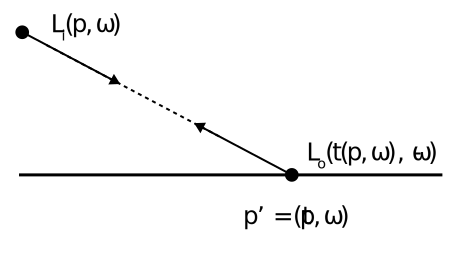
\includegraphics[width=\textwidth]{./radiance-along-ray.eps}
		\caption{在射线方向上的辐射量在空间中是不变的。所以如果有从$p$起始,沿着方向$\omega$的射线,我们想要计算沿着该射线的入射辐射,我们可以找到第一个相交的表面上的点$p^\prime$,并且计算从$p^\prime$处沿着方向$-\omega$的出射辐射来得到。射线投射函数$t(p,\omega)$给出了射线$(p,\omega)$相交的的第一个表面上的点$p^\prime$}
		\label{fig:radiance-along-ray}
		\end{framed}
	\end{figure}

	为了简洁我们可以丢弃掉下标,这样我们就可以将LTE写成:
	\begin{equation}
		L(p, \omega_o)=L_e(p, \omega_o)+\int_{S^2}f(p,\omega_o,\omega_i)L(t(p, \omega_i),-\omega_i)|\cos\theta_i|d\omega_i
		\label{eq:dir-int}
	\end{equation}
	
	上述表示的一个关键在于,我们只有一个需要关注的量$L$,即某表面上的点的出射辐射。
	当然,它出现在了方程的两边,所以我们的任务依然不轻松,但是它肯定比之前要好一点。
	我们之所以能够简化成这个方程,是因为我们强制保证了场景内的能量守恒,这一点是很重要的。
	
	\section{LTE的解析解}
	LTE的简洁具有一定迷惑性,事实上通常不可能去得到解析的解。
	基于物理的BSDF模型、随意的场景几何以及物体之间错综复杂的可见关系都鼓励我们采用数值方法。
	幸运的是,光线追踪算法和蒙特卡洛积分这对强有力的工具,可以完美地克服这些难点,而又不需要对LTE的不同组件去施加限制(比如说,要求所有的BSDF都是Lambertian或大大地限制所支持的几何表示)。
	
	在极度简单的设置下,找到LTE的解析解是可能的。
	尽管这对通用渲染没有任何帮助,但是可以帮助我们调试积分器的实现。
	如果一个应该完全解决LTE的积分器给出的结果与解析解对不上,那它肯定存在bug。
	作为一个例子,考虑在一个球体的内部,球体表面上的每一个点都有一个Lambertian BRDF,$f(p,\omega_0,\omega_i)=c$,同时对所有方向都有相同的发射辐射。那么我们有:
	\begin{equation*}
		L(p,\omega_o)=L_e+c\int_{H^2(n)}L(t(p,\omega_i),-\omega_i)|\cos\theta_i|d\omega_i
	\end{equation*}

	对于球体内每一个点,出射辐射的分布一定和每一个其他的点是一样的。
	对于不同的点,环境内没有任何东西能带来差异。
	所以每一个点的入射辐射也是一样的,同时$\cos$加权的入射辐射的积分也一定是相同的。
	这样,我们就可以把辐射方程全都换成常数,并进行简化 :
	\begin{equation*}
		L=L_e+c\pi L
	\end{equation*}

	我们可以马上地解出这个方程,但去考虑一下把L持续地代入方程的右边也是很有趣的。如果我们同时把$\pi c$替换成$\rho_{hh}$,即Lambertian表面的反射率,那么可以得到:
	\begin{equation*}
		\begin{split}
			L&=L_e+\rho_{hh}(L_e+\rho_{hh}(L_e+\cdots\\
			 &=\sum^\infty_{i=0}L_e\rho^i_{hh}
		\end{split}
	\end{equation*}

	换句话来说,出射辐射等于光源的发射辐射加上其经BSDF散射一次,再加上其经BSDF散射两次,再加上第三次,以此类推。

	由于能量守恒,$\rho_{hh}<1$,由级数收敛可以得出所有点在所有方向上所反射的辐射量是:
	\begin{equation*}
		L=\frac{L_e}{1-\rho_{hh}}
	\end{equation*}

	在通用情形下,重复地将入射辐射代入LTE方程的右边的过程也可以为我们带来一些启发性。比如说,\textit{DirectLightIntegrator}积分器通过做了一次代入来有效地计算结果:
	\begin{equation*}
		L(p,\omega_o)=L_e(p,\omega_o)+\int_{s^2}f(p,\omega_o,\omega_i)L_d|\cos\theta_i|d\omega_i
	\end{equation*}
	此时有:
	\begin{equation*}
		L_d=L_e(t(p,\omega_i),-\omega_i)
	\end{equation*}
	更深层的散射则被忽略了。

	在接下来的几页中,我们将会看到,按这种形式持续地代入方程右边,同时化简结果来表达LTE,会使我们更自然地发展渲染算法。
	
	\section{LTE的表面形式}	
	\eqref{eq:dir-int}如此复杂的一个原因是,场景中几何物体之间的关系在射线检测函数$t(p,\omega)$里是隐式的。
	如果将这个函数在积分式内的行为变得显式,这个方程的结构将会得到阐明。
	为了实现这个目标,我们将会把\eqref{eq:dir-int}重写成在对面积的积分而非对球体方向的积分。

	首先,我们定义从点$p^\prime$到点$p$的出射辐射函数:
	\begin{equation*}
		L(p^\prime\rightarrow p)=L(p^\prime,\omega)
	\end{equation*}
	如果$p^\prime$和$p$相互之间是可视的,而且$\omega=\widehat{p - p^\prime}$。
	我们同样可以表示$p^\prime$处的BSDF为:
	\begin{equation*}
		f(p^{\prime\prime}\rightarrow p^\prime\rightarrow p)=f(p^\prime,\omega_o,\omega_i)
	\end{equation*}
	这里$\omega_i=\widehat{p^{\prime\prime}-p^\prime}$,且$\omega_o=\widehat{p-p^\prime}$(图\ref{fig:three-point-form})
	\begin{figure}[h!]
		\begin{framed}
		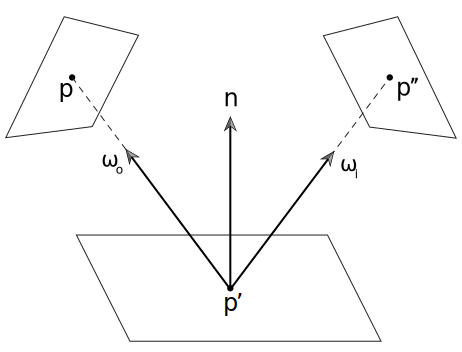
\includegraphics[width=\textwidth]{./three-point-form.eps}
		\caption{光传输方程的三点形式把积分式由对球体方向的积分转换成对场景内表面区域内的点的的积分。
		对把LTE推导成路径积分形式而言,这是一个关键的转换。}
		\label{fig:three-point-form}
		\end{framed}
	\end{figure}

	然而,仅仅把LTE的形式重写成这样是不对的。
	为了把LTE由对方向积分转换成对面积积分,我们还需要使其乘上体积角对面积的Jacobian行列式的绝对值,也就是$|\frac{\cos\theta^\prime}{r^2}|$。

	我们会把Jacobian行列式的绝对值、LTE中的$|\cos\theta|$以及一个二元可见函数$V$(如果两个点之间相互可见,那么$V=1$,否则$V=0$)全部组合进同一个几何函数$G(p\leftrightarrow p^\prime)$:
	\begin{equation*}
		G(p\leftrightarrow p^{\prime})=V(p\leftrightarrow p^{\prime})\frac{|\cos\theta||\cos\theta^{\prime}|}{||p-p^{\prime}||^2}
		\label{eq:b}
	\end{equation*}

	将这些函数代入光传输方程,同时转换成面积积分形式,我们就有:
	\begin{equation}
		L(p^\prime \rightarrow p)=L_e(p^\prime\rightarrow p)+\int_A f(p^{\prime\prime} \rightarrow p^\prime \rightarrow p)L(p^{\prime\prime}\rightarrow p^{\prime})G(p^{\prime\prime}\leftrightarrow p^\prime)dA(p^{\prime\prime})
		\label{eq:area-int}
	\end{equation}
	这里$A$是场景中所有的表面。
	
	虽然\eqref{eq:dir-int}和\eqref{eq:area-int}是等价的,但是它们用了两种不同的方式来传输光线。
	为了对\eqref{eq:dir-int}使用蒙特卡洛方法,我们可以根据球体上方向的分布来抽样许多方向,并沿着方向投射射线来进行积分。
	对于\eqref{eq:area-int}而言,我们却是根据表面面积的分布来选择一系列表面上的点,计算这些点之间的值来进行积分,通过投射射线来计算可见函数$V(p\leftrightarrow p^\prime)$。

	\section{对路径积分}
	有了面积积分形式的\eqref{eq:area-int},我们可以推导处一个更灵活的LTE形式,即光线传输的\textit{路径积分}。
	它将辐射表达为一个对路径的积分,这些路径本身也是在高维的\textit{路径空间}中的一个点。
	与像\eqref{eq:dir-int}一样由能量守恒笨拙地推出递归定义相反,使用路径空间可以给出一个可计算的对路径的显式积分。

	这个显式的形式使我们可以很自由地选择如何找到这些路径——本质上,任何随机选择路径的技术只要给定足够多的抽样数,都可以渲染出正确的结果,成为一种可用的渲染算法。这个形式的LTE也是将会在16章中提到的双向光线传输算法的基础。

	我们现在可以重复的展开三点形式的光线传输方程,重复地代入方程右边积分式中的的$L(p^{\prime\prime}\rightarrow p^\prime)$,以将面积积分式转换成涉及不同长度的路径积分形式:
	\begin{multline*}
		L\left(\mathrm{p}_{1} \rightarrow \mathrm{p}_{0}\right)= L_{\mathrm{e}}\left(\mathrm{p}_{1} \rightarrow \mathrm{p}_{0}\right)\\
		+\int_{A} L_{\mathrm{e}}\left(\mathrm{p}_{2} \rightarrow \mathrm{p}_{1}\right) f\left(\mathrm{p}_{2} \rightarrow \mathrm{p}_{1} \rightarrow \mathrm{p}_{0}\right) G\left(\mathrm{p}_{2} \leftrightarrow \mathrm{p}_{1}\right) \mathrm{d} A\left(\mathrm{p}_{2}\right) \\
		+\int_{A} \int_{A} L_{\mathrm{e}}\left(\mathrm{p}_{3} \rightarrow \mathrm{p}_{2}\right) f\left(\mathrm{p}_{3} \rightarrow \mathrm{p}_{2} \rightarrow \mathrm{p}_{1}\right) G\left(\mathrm{p}_{3} \leftrightarrow \mathrm{p}_{2}\right) \\
		\times f\left(\mathrm{p}_{2} \rightarrow \mathrm{p}_{1} \rightarrow \mathrm{p}_{0}\right) G\left(\mathrm{p}_{2} \leftrightarrow \mathrm{p}_{1}\right) \mathrm{d} A\left(\mathrm{p}_{3}\right) \mathrm{d} A\left(\mathrm{p}_{2}\right)+\cdots
	\end{multline*}

	右边相加的每一项都代表一段路径,长度是递增的。
	图\ref{fig:path-annotated-1}是第三项的一个例子,这条路径由四个顶点组成,由三个线段连接。
	第三项给出了长度为四的路径(第一个顶点在摄像机处,第二和第三个顶点在场景中的表面上,最后一个顶点在光源上)的所有贡献。
	这里的$p_0$和$p_1$已经由摄像机射线提前决定了,而$p_2$和$p_3$覆盖于场景中的所有表面上。
	对所有存在的$p_2$和$p_3$的积分给出了长度为四的路径对到达摄像机的辐射的贡献。
	\begin{figure}[h!]
		\begin{framed}
		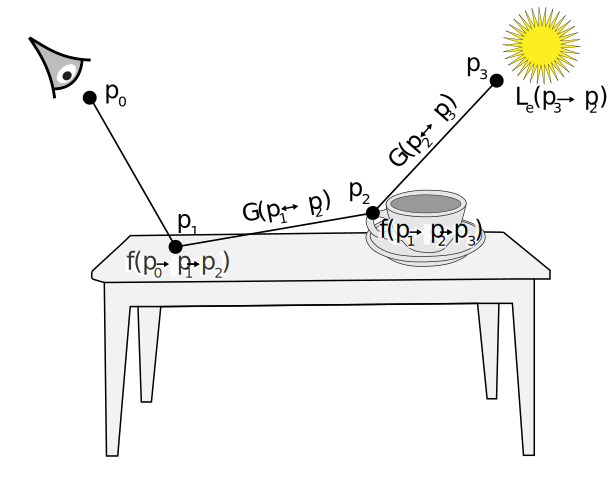
\includegraphics[width=\textwidth]{./path-annotated-1.eps}
		\caption{第三项中相乘的每一项被展示在这里:光源处的发射辐射$L_e$,两个顶点之间的几何函数$G$,以及由BSDF带来的散射项$f$}
		\label{fig:path-annotated-1}
		\end{framed}
	\end{figure}
	
	无限的求和可以被更紧凑地重写为:
	\begin{equation}
		L(p_1\rightarrow p_0)=\sum^\infty_{n=1}P(\overline{p}_n)
		\label{eq:compactly}
	\end{equation}
	$P(\overline{p}_n)$给出了路径$\overline{p}_n$所散射的辐射量,有$n+1$个顶点:
	\begin{equation*}
		\overline{p}_n=p_0,p_1,\ldots,p_n
	\end{equation*}
	其中$p_0$在图像平面上或透镜前,而$p_n$在光源上,并且:
	\begin{multline*}
	P\left(\overline{p}_{n}\right)=\underbrace{\int_{A} \int_{A} \cdots \int_{A} L_{\mathrm{e}}\left(\mathrm{p}_{n} \rightarrow \mathrm{p}_{n-1}\right)}_{n-1} \left(\prod_{i=1}^{n-1} f\left(\mathrm{p}_{i+1} \rightarrow \mathrm{p}_{i} \rightarrow \mathrm{p}_{i-1}\right) G\left(\mathrm{p}_{i+1} \leftrightarrow \mathrm{p}_{i}\right)\right) \\
	\times \mathrm{d} A\left(\mathrm{p}_{2}\right) \cdots \mathrm{d} A\left(\mathrm{p}_{n}\right)
	\end{multline*}

	在我们继续之前,我们先定义一个额外的函数,它能帮助我们进行接下来的讨论。
	几何函数与路径的BSDF的乘积被称为路径的\textit{通量}。
	它描述了来自光源的经过期间所有顶点的散射后到达摄像机的辐射量的比例。我们定义为:
	\begin{equation*}
		T(\overline{p}_n)=\prod^{n-1}_{i=1}f(p_{i+1}\rightarrow p_i \rightarrow p_{i-1})G(p_{i+1} \leftrightarrow p_i)
	\end{equation*}
	所以:
	\begin{equation*}
		P(\overline{p}_n)=\underbrace{\int_A\int_A\cdots\int_A}_{n-1}L_e(p_n\rightarrow p_{n-1})T(\overline{p}_n)dA(p_2)\cdots dA(p_n)
	\end{equation*}

	有了\eqref{eq:compactly}和给定的长度$n$, 假如想要针对长度为$n$的路径计算到达$p_0$的辐射量的蒙特卡洛估计,我们只需要以合适的抽样密度去抽样一系列场景中的顶点,生成路径,用这些顶点来估计$P(\overline{p}_n)$的值。
	无论我们生成的路径顶点是从摄像机开始、从光源开始、同时从摄像机和光源开始还是从中间的某一个点开始,都只会影响蒙特卡洛估计中权值的计算方式。
	我们会在这章和之后的两章中看到看到这个公式如何产生实用的光线传输算法。

	\section{积分式中的Delta分布}
	$P(\overline{p}_i)$的主体中可能包含delta函数,包括由delta分布组成的BSDF和特定的光源种类(比如说,点光源和平行光源)。
	如果包含的话,光线传输算法必须显式地处理这些delta分布。
	打个比方,从表面上的一点随机的选择一个方向,并祈祷这条射线能与一个点光源相交,这是不可能的。
	所以,如果我们想包含这种分布的话,我们必须要选择单一的朝向光源的方向。
	(抽样存在delta组件的BSDF也是一样的。)
	虽然处理这种情况会给积分器的实现带来额外的复杂性,但是这是值得的,因为他可以降低积分式的维度,将其中的一部分变成简单的求和。

	举个例子,考虑一个直接照明(长度为2,这样只需要考虑摄像机射线所相交的第一个点的直接光照)公式$P(\overline{p}_2)$,和场景中的一个由delta分布表达的点光源$p_{\mathrm{light}}$:
	\begin{align*}
		P\left(\overline{\mathrm{p}}_{2}\right) &=\int_{A} L_{\mathrm{e}}\left(\mathrm{p}_{2} \rightarrow \mathrm{p}_{1}\right) f\left(\mathrm{p}_{2} \rightarrow \mathrm{p}_{1} \rightarrow \mathrm{p}_{0}\right) G\left(\mathrm{p}_{2} \leftrightarrow \mathrm{p}_{1}\right) \mathrm{d} A\left(\mathrm{p}_{2}\right) \\
		&=\frac{\delta\left(\mathrm{p}_{\mathrm{light}}-\mathrm{p}_{2}\right) L_{\mathrm{e}}\left(\mathrm{p}_{\mathrm{light}} \rightarrow \mathrm{p}_{1}\right)}{p\left(\mathrm{p}_{\mathrm{light}}\right)} f\left(\mathrm{p}_{2} \rightarrow \mathrm{p}_{1} \rightarrow \mathrm{p}_{0}\right) G\left(\mathrm{p}_{2} \leftrightarrow \mathrm{p}_{1}\right)
	\end{align*}

	换句话说,$p_2$必须与点光源的位置相等。
	分子中的delta函数被消掉了,因为分母中的$p(p_{\mathrm{light}})$隐式包含一个delta函数,这样我们就只剩下一个可以直接计算的公式,不再需要蒙特卡洛。
	路径通量$T(\overline{p}_n)$中含有delta函数的BSDF有着同样的处境,它们都同样消除了对面积的积分,使其可以直接计算。

	\section{分割积分式}
	至今为止,被开发出来的许多渲染算法都只能在特定的条件下才能很好地解决LTE。比如说,Whitted积分器只能处理delta BSDF中的specular反射,而忽略了其他的多重散射光,包括diffuse和glossy的BSDF。
	16.2.2章节会介绍一些密度估计的概念,它们是用来实现一个叫作\textit{随机渐进光子映射}(SPPM)的渲染算法的,
	而那个算法所使用的密度估计之所以能够在diffuse表面上带来很好的效果,是因为散射的辐射量只依赖于表面的位置,所以只需要存储一个2d辐射的离散表。
	但是当要处理glossy表面时,其他的技术比如路径追踪会更适合。
	
	因为我们想要推导的是处理所有的,而非忽略或重复计算散射模式的光线传输算法,所以,仔细地搞明白特定的算法属于LTE的哪一部分是很重要的。
	一个很好的方法是将LTE分割成好几部分,比如说,我们可以将路径的求和部分展开为:
	\begin{equation*}
		L\left(\mathrm{p}_{1} \rightarrow \mathrm{p}_{0}\right)=P\left(\overline{\mathrm{p}}_{1}\right)+P\left(\overline{\mathrm{p}}_{2}\right)+\sum_{i=3}^{\infty} P\left(\overline{\mathrm{p}}_{i}\right)
	\end{equation*}
	第一项可以简单地计算$p_1$的发射辐射,第二项可以由精确的直接光照算法技术来解决。
	剩下的项可以采用较快但是不精确的方法,如果这些附加的项对于所有的辐射量而言的贡献非常小,那么这是一个值得接受的妥协。
	特别需要注意的一点是,算法必须小心地保证$P(\overline{p}_1)$和$P(\overline{p}_2)$中没有包含涉及$P(\overline{p}_3)$以及其余的项的部分。

	分割独立的$P(\overline{p}_n)$项也是很有用的。
	比如说,我们可能想要将发射辐射的项分割成来自较小的光源的$L_{e,s}$和来自较大的光源的$L_{e,l}$,给出两个分离的积分式:
	\begin{equation*}
		\begin{aligned}
			P\left(\overline{p}_{n}\right)=& \int_{A^{n-1}}\left(L_{\mathrm{e}, \mathrm{s}}\left(\mathrm{p}_{n} \rightarrow \mathrm{p}_{n-1}\right)+L_{\mathrm{e}, 1}\left(\mathrm{p}_{\mathrm{n}} \rightarrow \mathrm{p}_{\mathrm{n}-1}\right)\right) T\left(\overline{\mathrm{p}}_{n}\right) \mathrm{d} A\left(\mathrm{p}_{2}\right) \cdots \mathrm{d} A\left(\mathrm{p}_{n}\right) \\
			=& \int_{A^{n-1}} L_{\mathrm{e}, \mathrm{s}}\left(\mathrm{p}_{\mathrm{n}} \rightarrow \mathrm{p}_{\mathrm{n}-1}\right) T\left(\overline{\mathrm{p}}_{n}\right) \mathrm{d} A\left(\mathrm{p}_{2}\right) \cdots \mathrm{d} A\left(\mathrm{p}_{n}\right) \\
			&+\int_{A^{n-1}} L_{\mathrm{e}, 1}\left(\mathrm{p}_{\mathrm{n}} \rightarrow \mathrm{p}_{\mathrm{n}-1}\right) T\left(\overline{\mathrm{p}}_{n}\right) \mathrm{d} A\left(\mathrm{p}_{2}\right) \cdots \mathrm{d} A\left(\mathrm{p}_{n}\right)
		\end{aligned}
	\end{equation*}
	这两个积分式可以被独立计算,可能使用完全不同的算法或不同的抽样数,使其可以很好地处理不同的情况。
	只要$L_{e,s}$积分式忽略了大光源,且$L_{e,l}$忽略了小光源,那么所有的光源都被正确分类为了“小”或者“大”,最终就可以计算出正确的结果。

	当然,BSDF的项也可以被分割(事实上,在章节8.1中介绍的将BSDF分类为不同的BxDFType,正是应用了这个方法)。
	比如说,如果将BSDF由delta函数所表示的组件记作$f_{\Delta}$,把其余的组件记作$f_{\neg\Delta}$,那么:
	\begin{multline*}
		P\left(\overline{\mathrm{p}}_{n}\right)=\int_{A^{n-1}} L_{\mathrm{e}}\left(\mathrm{p}_{\mathrm{n}} \rightarrow \mathrm{p}_{\mathrm{n}-1}\right) \\
		\times \prod_{i=1}^{n-1}\left(f_{\Delta}\left(\mathrm{p}_{\mathrm{i}+1} \rightarrow \mathrm{p}_{\mathrm{i}} \rightarrow \mathrm{p}_{\mathrm{i}-1}\right)+f_{\neg \Delta}\left(\mathrm{p}_{\mathrm{i}+1} \rightarrow \mathrm{p}_{\mathrm{i}} \rightarrow \mathrm{p}_{\mathrm{i}-1}\right)\right) \\
		\times G\left(\mathrm{p}_{\mathrm{i}+1} \leftrightarrow \mathrm{p}_{\mathrm{i}}\right) \mathrm{d} A\left(\mathrm{p}_{2}\right) \cdots \mathrm{d} A\left(\mathrm{p}_{\mathrm{n}}\right)
	\end{multline*}
	需要注意的是,因为在连乘中有$n-1$项BSDF,千万不能只单独考虑包含$f_{\Delta}$的项或是只单独考虑包含$f_{\neg\Delta}$的项。
	如果使用了这样的分割模式,所有类似于$f_\Delta f_{\neg\Delta}f_{\neg\Delta}$的项都必须考虑到。
\end{document}
